\documentclass[12pt]{article}
\usepackage{booktabs}
\usepackage{tabularx}
\usepackage{caption}
\usepackage{nameref}
\usepackage{graphicx}
\usepackage{float}
% поддержка кириллицы
\usepackage[T2A]{fontenc}   % шрифтовая кодировка
\usepackage[utf8]{inputenc} % кодировка исходного файла (UTF-8)
\usepackage[main=russian,english]{babel} % языки: основной русский, доп. английский
\usepackage{amsmath}
\usepackage{breqn}

\title{Использование множественных измерений в таксономических задачах}
\author{Р. А. Фишер,\\
  {\small доктор наук,}\\ 
  {\small член Лондонского королевского общества}}
\date{}

\renewcommand{\thetable}{\Roman{table}}
\makeatletter
\renewcommand{\@seccntformat}[1]{\csname the#1\endcsname\hspace{0.5em}}
\makeatother

\begin{document}

\maketitle

\begin{abstract}
Эта работа написана для иллюстрации практического численного примера из области растительной таксономии, где понятие дискриминантной функции, по-видимому, может оказать непосредственную пользу.
\end{abstract}
\section{Дискриминантные функции}

Когда две или более популяции измерены по нескольким признакам 
\[
x_1, \dots, x_s,
\] особый интерес представляют определённые линейные функции этих измерений, с помощью которых популяции лучше всего различаются. По предложению автора уже было использовано это обстоятельство в краниометрии: ($a$) мистером Э. С. Мартином, который применил принцип к половым различиям в измерениях нижней челюсти, и ($b$) мисс Милдред Барнард, которая показала, как из серии датированных наборов получить особую комбинацию черепных измерений, наиболее явно демонстрирующую прогрессивную или секулярную тенденцию. В настоящей работе применение того же принципа будет проиллюстрировано на таксономической задаче; также будут обсуждены некоторые вопросы, связанные с точностью применяемых процедур.

\section{Арифметическая процедура}

В Таблице~\ref{tab:1} приведены измерения цветков по пятидесяти растениям каждого из двух видов \textit{Iris setosa} и \textit{I. versicolor}, растущих вместе в одной колонии и измеренных доктором Э. Андерсоном, которому я обязан за предоставленные данные. Приведены четыре измерения цветка.


Сначала рассмотрим вопрос: какую линейную функцию четырёх измерений
\[
X = \lambda_{1} x_{1} + \lambda_{2} x_{2} + \lambda_{3} x_{3} + \lambda_{4} x_{4}
\]
следует выбрать, чтобы максимизировать отношение разности между средними значениями видов к стандартному отклонению внутри видов? Наблюдаемые средние значения и их различия приведены в Таблице~\ref{tab:2}. Разности можно обозначить через $d_p$, где \text{$p = 1,\,2,\,3 \text{ или } 4$} для четырёх измерений.



Суммы квадратов и произведений отклонений от средних значений каждого вида показаны в Таблице~\ref{tab:3}. Поскольку использовались по пятьдесят растений каждого вида, эти суммы содержат 98 степеней свободы. Эти суммы квадратов или произведений можно обозначить через $S_{pq}$, где $p$ и $q$ независимо принимают значения \text{$1,\,2,\,3 \text{ и } 4$}.


Тогда для любой линейной функции $X$ измерений, определённой выше, разность между средними значениями $X$ у двух видов равна

\[
D = \lambda_{1} d_{1} + \lambda_{2} d_{2} + \lambda_{3} d_{3} + \lambda_{4} d_{4}
\] в то время как дисперсия $X$ внутри видов пропорциональна

\[
S = \sum_{p=1}^{4}\sum_{q=1}^{4} \lambda_{p} \lambda_{q} S_{pq}
\].


Особая линейная функция, которая наилучшим образом различает два вида, будет той, для которой отношение $D^2/S$ максимально, при независимом изменении четырёх коэффициентов $\lambda_{1}$, $\lambda_{2}$, $\lambda_{3}$ и $\lambda_{4}$. Это даёт для каждого $\lambda$


\[
\frac{D}{S^2} \biggl\{ 2S \frac{\partial D}{\partial \lambda} - D \frac{\partial S}{\partial \lambda} \biggl\} = 0,
\] или

{
\setlength{\tabcolsep}{2pt}
\begin{table}[H]
\centering
\scriptsize
\caption{}
\label{tab:1}
\begin{tabularx}{\textwidth}{|*{12}{>{\centering\arraybackslash}X|}}
\hline
\multicolumn{4}{|c|}{\textit{Iris setosa}} &
\multicolumn{4}{c|}{\textit{Iris versicolor}} &
\multicolumn{4}{c|}{\textit{Iris virginica}} \\
\hline
\multicolumn{2}{|c|}{Чашелистик} &
\multicolumn{2}{c|}{Лепесток} &
\multicolumn{2}{c|}{Чашелистик} &
\multicolumn{2}{c|}{Лепесток} &
\multicolumn{2}{c|}{Чашелистик} &
\multicolumn{2}{c|}{Лепесток} \\
\hline
\tiny{Длина} & \tiny{Ширина} & \tiny{Длина} & \tiny{Ширина} &
\tiny{Длина} & \tiny{Ширина} & \tiny{Длина} & \tiny{Ширина} &
\tiny{Длина} & \tiny{Ширина} & \tiny{Длина} & \tiny{Ширина} \\
\hline
5.1 & 3.5 & 1.4 & 0.2 & 7.0 & 3.2 & 4.7 & 1.4 & 6.3 & 3.3 & 6.0 & 2.5 \\
4.9 & 3.0 & 1.4 & 0.2 & 6.4 & 3.2 & 4.5 & 1.5 & 5.8 & 2.7 & 5.1 & 1.9 \\
4.7 & 3.2 & 1.3 & 0.2 & 6.9 & 3.1 & 4.9 & 1.5 & 7.1 & 3.0 & 5.9 & 2.1 \\
4.6 & 3.1 & 1.5 & 0.2 & 5.5 & 2.3 & 4.0 & 1.3 & 6.3 & 2.9 & 5.6 & 1.8 \\
5.0 & 3.6 & 1.4 & 0.2 & 6.5 & 2.8 & 4.6 & 1.5 & 6.5 & 3.0 & 5.8 & 2.2 \\
5.4 & 3.9 & 1.7 & 0.4 & 5.7 & 2.8 & 4.5 & 1.3 & 7.6 & 3.0 & 6.6 & 2.1 \\
4.6 & 3.4 & 1.4 & 0.3 & 6.3 & 3.3 & 4.7 & 1.6 & 4.9 & 2.5 & 4.5 & 1.7 \\
5.0 & 3.4 & 1.5 & 0.2 & 4.9 & 2.4 & 3.3 & 1.0 & 7.3 & 2.9 & 6.3 & 1.8 \\
4.4 & 2.9 & 1.4 & 0.2 & 6.6 & 2.9 & 4.6 & 1.3 & 6.7 & 2.5 & 5.8 & 1.8 \\
4.9 & 3.1 & 1.5 & 0.1 & 5.2 & 2.7 & 3.9 & 1.4 & 7.2 & 3.6 & 6.1 & 2.5 \\
5.4 & 3.7 & 1.5 & 0.2 & 5.0 & 2.0 & 3.5 & 1.0 & 6.5 & 3.2 & 5.1 & 2.0 \\
4.8 & 3.4 & 1.6 & 0.2 & 5.9 & 3.0 & 4.2 & 1.5 & 6.4 & 2.7 & 5.3 & 1.9 \\
4.8 & 3.0 & 1.4 & 0.1 & 6.0 & 2.2 & 4.0 & 1.0 & 6.8 & 3.0 & 5.5 & 2.1 \\
4.3 & 3.0 & 1.1 & 0.1 & 6.1 & 2.9 & 4.7 & 1.4 & 5.7 & 2.5 & 5.0 & 2.0 \\
5.8 & 4.0 & 1.2 & 0.2 & 5.6 & 2.9 & 3.6 & 1.3 & 5.8 & 2.8 & 5.1 & 2.4 \\
5.7 & 4.4 & 1.5 & 0.4 & 6.7 & 3.1 & 4.4 & 1.4 & 6.4 & 3.2 & 5.3 & 2.3 \\
5.4 & 3.9 & 1.3 & 0.4 & 5.6 & 3.0 & 4.5 & 1.5 & 6.5 & 3.0 & 5.5 & 1.8 \\
5.1 & 3.5 & 1.4 & 0.3 & 5.8 & 2.7 & 4.1 & 1.0 & 7.7 & 3.8 & 6.7 & 2.2 \\
5.7 & 3.8 & 1.7 & 0.3 & 6.2 & 2.2 & 4.5 & 1.5 & 7.7 & 2.6 & 6.9 & 2.3 \\
5.1 & 3.8 & 1.5 & 0.3 & 5.6 & 2.5 & 3.9 & 1.1 & 6.0 & 2.2 & 5.0 & 1.5 \\
5.4 & 3.4 & 1.7 & 0.2 & 5.9 & 3.2 & 4.8 & 1.8 & 6.9 & 3.2 & 5.7 & 2.3 \\
5.1 & 3.7 & 1.5 & 0.4 & 6.1 & 2.8 & 4.0 & 1.3 & 5.6 & 2.8 & 4.9 & 2.0 \\
4.6 & 3.6 & 1.0 & 0.2 & 6.3 & 2.5 & 4.9 & 1.5 & 7.7 & 2.8 & 6.7 & 2.0 \\
5.1 & 3.3 & 1.7 & 0.5 & 6.1 & 2.8 & 4.7 & 1.2 & 6.3 & 2.7 & 4.9 & 1.8 \\
4.8 & 3.4 & 1.9 & 0.2 & 6.4 & 2.9 & 4.3 & 1.3 & 6.7 & 3.3 & 5.7 & 2.1 \\
5.0 & 3.0 & 1.6 & 0.2 & 6.6 & 3.0 & 4.4 & 1.4 & 7.2 & 3.2 & 6.0 & 1.8 \\
5.0 & 3.4 & 1.6 & 0.4 & 6.8 & 2.8 & 4.8 & 1.4 & 6.2 & 2.8 & 4.8 & 1.8 \\
5.2 & 3.5 & 1.5 & 0.2 & 6.7 & 3.0 & 5.0 & 1.7 & 6.1 & 3.0 & 4.9 & 1.8 \\
5.2 & 3.4 & 1.4 & 0.2 & 6.0 & 2.9 & 4.5 & 1.5 & 6.4 & 2.8 & 5.6 & 2.1 \\
4.7 & 3.2 & 1.6 & 0.2 & 5.7 & 2.6 & 3.5 & 1.0 & 7.2 & 3.0 & 5.8 & 1.6 \\
4.8 & 3.1 & 1.6 & 0.2 & 5.5 & 2.4 & 3.8 & 1.1 & 7.4 & 2.8 & 6.1 & 1.9 \\
5.4 & 3.4 & 1.5 & 0.4 & 5.5 & 2.4 & 3.7 & 1.0 & 7.9 & 3.8 & 6.4 & 2.0 \\
5.2 & 4.1 & 1.5 & 0.1 & 5.8 & 2.7 & 3.9 & 1.2 & 6.4 & 2.8 & 5.6 & 2.2 \\
5.5 & 4.2 & 1.4 & 0.2 & 6.0 & 2.7 & 5.1 & 1.6 & 6.3 & 2.8 & 5.1 & 1.5 \\
4.9 & 3.1 & 1.5 & 0.1 & 5.4 & 3.0 & 4.5 & 1.5 & 6.1 & 2.6 & 5.6 & 1.4 \\
5.0 & 3.2 & 1.2 & 0.2 & 6.0 & 3.4 & 4.5 & 1.6 & 7.7 & 3.0 & 6.1 & 2.3 \\
5.5 & 3.5 & 1.3 & 0.2 & 6.7 & 3.1 & 4.7 & 1.5 & 6.3 & 3.4 & 5.6 & 2.4 \\
4.9 & 3.1 & 1.5 & 0.1 & 6.3 & 2.3 & 4.4 & 1.3 & 6.4 & 3.1 & 5.5 & 1.8 \\
4.4 & 3.0 & 1.3 & 0.2 & 5.6 & 3.0 & 4.1 & 1.3 & 6.0 & 3.0 & 4.8 & 1.8 \\
5.1 & 3.4 & 1.5 & 0.2 & 5.5 & 2.5 & 4.0 & 1.3 & 6.9 & 3.1 & 5.4 & 2.1 \\
5.0 & 3.5 & 1.3 & 0.3 & 5.5 & 2.6 & 4.4 & 1.2 & 6.7 & 3.1 & 5.6 & 2.4 \\
4.5 & 2.3 & 1.3 & 0.3 & 6.1 & 3.0 & 4.6 & 1.4 & 6.9 & 3.1 & 5.1 & 2.3 \\
4.4 & 3.2 & 1.3 & 0.2 & 5.8 & 2.6 & 4.0 & 1.2 & 5.8 & 2.7 & 5.1 & 1.9 \\
5.0 & 3.5 & 1.6 & 0.6 & 5.0 & 2.3 & 3.3 & 1.0 & 6.8 & 3.2 & 5.9 & 2.3 \\
5.1 & 3.8 & 1.9 & 0.4 & 5.6 & 2.7 & 4.2 & 1.3 & 6.7 & 3.3 & 5.7 & 2.5 \\
4.8 & 3.0 & 1.4 & 0.3 & 5.7 & 3.0 & 4.2 & 1.2 & 6.7 & 3.0 & 5.2 & 2.3 \\
5.1 & 3.8 & 1.6 & 0.2 & 5.7 & 2.9 & 4.2 & 1.3 & 6.3 & 2.5 & 5.0 & 1.9 \\
4.6 & 3.2 & 1.4 & 0.2 & 6.2 & 2.9 & 4.3 & 1.3 & 6.5 & 3.0 & 5.2 & 2.0 \\
5.3 & 3.7 & 1.5 & 0.2 & 5.1 & 2.5 & 3.0 & 1.1 & 6.2 & 3.4 & 5.4 & 2.3 \\
5.0 & 3.3 & 1.4 & 0.2 & 5.7 & 2.8 & 4.1 & 1.3 & 5.9 & 3.0 & 5.1 & 1.8 \\
\hline
\end{tabularx}
\end{table}
}

\begin{table}[H]
\centering
\footnotesize
\caption[Статистические методы]{Наблюдаемые средние значения для двух видов и их разность, см}
\label{tab:2}
\begin{tabularx}{\textwidth}{|>{\raggedright\arraybackslash}p{5cm} 
                               |>{\centering\arraybackslash}X
                               |>{\centering\arraybackslash}X
                               |>{\centering\arraybackslash}X|}
\hline
 & \textit{versicolor} & \textit{setosa} & Разность ($V-S$) \\
\hline
Длина чашелистика ($x_1$) & 5.936 & 5.006 & 0.930 \\
Ширина чашелистика ($x_2$)  & 2.770 & 3.428 & $-0.658$ \\
Длина лепестка ($x_3$) & 4.260 & 1.462 & 2.798 \\
Ширина лепестка ($x_4$)  & 1.326 & 0.246 & 1.080 \\
\hline
\end{tabularx}
\end{table}

\begin{table}[H]
\centering
\footnotesize
\caption{Суммы квадратов и произведений четырёх измерений внутри видов, см$^2$}
\label{tab:3}
\begin{tabularx}{\textwidth}{|>{\raggedright\arraybackslash}p{3.7cm} 
                               |>{\centering\arraybackslash}X
                               |>{\centering\arraybackslash}X
                               |>{\centering\arraybackslash}X
                               |>{\centering\arraybackslash}X|}

\hline
 & Длина чашелистика & Ширина чашелистика & Длина лепестка & Ширина лепестка \\
\hline
Длина чашелистика & 19.1434 & 9.0356  & 9.7634  & 3.2394 \\
Ширина чашелистика  & 9.0356  & 11.8658 & 4.6232  & 2.4746 \\
Длина лепестка & 9.7634  & 4.6232  & 12.2978 & 3.8794 \\
Ширина лепестка  & 3.2394  & 2.4746  & 3.8794  & 2.4604 \\
\hline
\end{tabularx}
\end{table}


\[
\frac{1}{2} \frac{\partial S}{\partial \lambda} = 
\frac{S}{D} \frac{\partial D}{\partial \lambda},
\] где можно заметить, что $S/D$ является постоянным множителем для четырёх неизвестных коэффициентов. Следовательно, требуемые коэффициенты пропорциональны решениям системы уравнений


\begin{equation} \label{eq:1}
\left.
\begin{aligned}
S_{11} \lambda_{1} + S_{12} \lambda_{2} + S_{13} \lambda_{3} + S_{14} \lambda_{4} &= d_1 ,\\
S_{21} \lambda_{1} + S_{22} \lambda_{2} + S_{23} \lambda_{3} + S_{24} \lambda_{4} &= d_2 ,\\
S_{31} \lambda_{1} + S_{32} \lambda_{2} + S_{33} \lambda_{3} + S_{34} \lambda_{4} &= d_3 ,\\
S_{41} \lambda_{1} + S_{42} \lambda_{2} + S_{43} \lambda_{3} + S_{44} \lambda_{4} &= d_4 .
\end{aligned}
\right\}
\end{equation}



Если, в свою очередь, подставить единицу для каждой из разностей и ноль для остальных, полученные решения составляют матрицу множителей, обратную матрице $S$; численно мы находим:


\begin{table}[H]
\centering
\footnotesize
\caption{Матрица множителей, обратная суммам квадратов и произведений внутри видов (см$^{-2}$).}
\label{tab:4}
\begin{tabularx}{\textwidth}{|>{\raggedright\arraybackslash}p{3.7cm} 
                               |>{\centering\arraybackslash}X
                               |>{\centering\arraybackslash}X
                               |>{\centering\arraybackslash}X
                               |>{\centering\arraybackslash}X|}\hline
 & Длина чашелистика & Ширина чашелистика & Длина лепестка & Ширина лепестка \\
\hline
Длина чашелистика &  0.1187161 & -0.0668666 & -0.0816158 &  0.0396350 \\
Ширина чашелистика  & -0.0668666 &  0.1452736 &  0.0334101 & -0.1107529 \\
Длина лепестка & -0.0816158 &  0.0334101 &  0.2193614 & -0.2720206 \\
Ширина лепестка  &  0.0396350 & -0.1107529 & -0.2720206 &  0.8945506 \\
\hline
\end{tabularx}
\end{table}
Эти значения можно обозначить как $s_{pq}$ для $p$ и $q$ от 1 до 4.

Умножив столбцы матрицы из Таблицы~\ref{tab:4} на наблюдаемые разности, получаем
решения уравнения \eqref{eq:1} в виде
\[
\lambda_{1}=-0.0311511, \lambda_{2}=-0.1839075, \lambda_{3}=+0.2221044, \lambda_{4}=+0.3147370,
\]
так что, если принять коэффициент длины чашелистика за единицу, требуемая составная
величина равна
\[
X = x_1 + 5.9037 x_2 - 7.1299 x_3 - 10.1036 x_4.
\] 
Если в этом выражении подставить наблюдаемые значения у растений \textit{setosa}, среднее, вычисленное по данным из Таблицы~\ref{tab:1}, будет
\[
5.006 + (3.428)(5.9037) - (1.462)(7.1299) - (0.246)(10.1036) = 12.3345\ \text{см};
\] 
для \textit{versicolor}, наоборот, имеем
\[
5.936 + (2.770)(5.9037) - (4.260)(7.1299) - (1.326)(10.1036) = -21.4815\ \text{см}.
\] 
Разность средних значений составной величины таким образом равна 33.816 см.

Явность метрических признаков двух видов теперь можно оценить, сравнив эту разность средних со стандартной ошибкой. Используя значения из Таблицы~\ref{tab:3} с коэффициентами нашей составной величины, получаем

{\small
\[
\begin{aligned}
19.1431 + (9.0356)(5.9037) - (9.7634)(7.1299) - (3.2394)(10.1036) &= -29.8508,\\
9.0356 + (11.8658)(5.9037) - (4.6232)(7.1299) - (2.4746)(10.1036) &= 21.1224,\\
9.7634 + (4.6232)(5.9037) - (12.2978)(7.1299) - (3.8794)(10.1036) &= -89.8206,\\
3.2394 + (2.4746)(5.9037) - (3.8794)(7.1299) - (2.4604)(10.1036) &= -34.6699,
\end{aligned}
\] } и, наконец, 
{\small
\[
-29.8508 + (21.1224)(5.9037) + (89.8206)(7.1299) + (34.6699)(10.1036) = 1085.5522.
\] }

Среднюю дисперсию двух видов по составной величине можно оценить, разделив это значение (1085.5522) на 95; дисперсию разности между двумя средними по пятидесяти растениям каждого вида — разделив снова на 25. Для одного растения дисперсия равна 11.4269, так что средняя разность 33.816 см между парой растений разных видов имеет стандартное отклонение 4.781 см. Для средних по пятидесяти растениям та же средняя разность имеет стандартную ошибку 0.6761 см, что составляет примерно одну пятидесятую от её значения.
\section{Интерпретация}

Отношение разности средних выбранной составной величины к её стандартной ошибке для отдельных растений также представляет интерес в связи с вероятностью ошибочной классификации, если природа вида оценивалась бы исключительно по измерениям.  
По причинам, которые будут обсуждены далее, дисперсию одного растения мы оценим, разделив 1085.5522 на 95, получив 11.4269 см$^2$ для дисперсии и 3.3804 см для стандартного отклонения. Предположим, что растение классифицировано неверно, если его отклонение в правильном направлении превышает половину разности, 33.816 см, между видами; отношение к стандартному отклонению, как оценено, равно 5.0018.

Таблица нормального распределения (\textit{\nameref{tab:2}}, Таблица~\ref{tab:2}) показывает, что отношение 4.89164 превышается пять раз на миллион, а 5.32672 — только один раз на два миллиона испытаний.  
По логарифмической интерполяции частота, соответствующая отношению 5.0018, составляет примерно 2.79 на миллион.  
Если дисперсии двух видов не равны, эта частота несколько переоценивается данным методом, поскольку следует делить специфическую разность пропорционально двум стандартным отклонениям, а при постоянной сумме дисперсий сумма стандартных отклонений наибольшая, когда они равны.  
Следовательно, можно сразу заключить, что если измерения распределены почти нормально, вероятность ошибочной классификации, используя только составную величину, составляет менее трёх на миллион.

То же отношение интересно и с другой стороны. Если выбранная составная величина $X$ анализируется с точки зрения её вариации внутри и между видами, сумма квадратов между видами должна быть равна $25 D^2$.  
Численно мы имеем, следовательно,

\begin{table}[H]
\centering
\footnotesize
\caption{Анализ дисперсии выбранной составной величины $X$, между и внутри видов}
\label{tab:5}
\begin{tabular}{|c|c|c|}
\hline
 & Степени свободы & Сумма квадратов \\
\hline
Между видами & 4  & 28588.05 \\
Внутри видов  & 95 & 1085.55  \\
\hline
Итого         & 99 & 29673.60 \\
\hline
\end{tabular}
\end{table}
Из общей суммы только 3.6583\% приходится на внутривидовую вариацию, а 96.3417\% — на межвидовую.  
Составная величина выбрана так, чтобы максимизировать последнюю долю. Поскольку, кроме специфических средних, мы использовали три настраиваемых коэффициента, вариация внутри видов содержит лишь 95 степеней свободы.

При составлении вариативной величины $X$ мы умножили исходные значения $\lambda$ на -32.1018, чтобы придать измерению длины чашелистика коэффициент, равный единице.  
Если бы мы использовали исходные значения, анализ из Таблицы~\ref{tab:5} выглядел бы следующим образом:

\begin{table}[H]
\centering
\footnotesize
\caption{Анализ дисперсии исходной составной величины $X$, между и внутри видов}
\label{tab:6}
\begin{tabular}{|c|c|c|c|}
\hline
 & Степени свободы & Сумма квадратов & \\
\hline
Между видами & 4  & 27.74160 & $=25 D^2$ \\
Внутри видов  & 95 & 1.05341  & $=D=S$ \\
\hline
Итого         & 99 & 28.79501 & $D(1+25D)$ \\
\hline
\end{tabular}
\end{table}

При умножении уравнений \eqref{eq:1} на $\lambda_{1}$, $\lambda_{2}$, $\lambda_{3}$ и $\lambda_{4}$ и последующем сложении оказывается, что
$S = \sum{\lambda d} = D$, то есть специфическая разность в исходной составной величине $X$.  
Долю суммы квадратов внутри видов (3.6 \%) можно было бы найти просто как $1 / (1 + 25 D)$.

\section{Аналогия частичной регрессии}

Анализ Таблицы~\ref{tab:6} наводит на интересную аналогию. Если каждому растению присвоить значение вариативной величины $y$, одинаковое для всех представителей одного вида, анализ дисперсии $y$, между частями, объясняемыми линейной регрессией по измерениям
$x_{1}, \ldots, x_{4}$, и остаточная вариация после подгонки такой регрессии будут идентичны Таблице~\ref{tab:6}, если $y$ задать соответствующие равные и противоположные значения для двух видов.

В общем случае, при различном числе представителей двух видов, $n_{1}$ и $n_{2}$, если значения $y$, присвоенные растениям, равны
\[
\frac{n_{2}}{n_{1}+n_{2}} \quad \text{и} \quad \frac{- n_{1}}{n_{1}+n_{2}},
\]
отличаясь на единицу, правые части уравнений для коэффициентов регрессии, соответствующих уравнению \eqref{eq:1}, будут
\[
\frac{n_{1}n_{2}}{n_{1}+n_{2}} d_{p},
\]
где $d_{p}$ — разность средних двух видов по любому из измерений.  
Типичный коэффициент левой части будет
\[
S_{pq} + \frac{n_{1}n_{2}}{n_{1}+n_{2}} d_{p} d_{q}.
\]

Перенеся дополнительные дроби в правую часть, мы получим уравнения, идентичные \eqref{eq:1}, за исключением того, что правые части теперь равны

\[
\frac{n_{1}n_{2}}{n_{1}+n_{2}} d_{p} \, (1 - \sum \lambda' d),
\]
где $\lambda'$ обозначает решение новых уравнений; следовательно
\[
\lambda' = \frac{n_{1}n_{2}}{n_{1}+n_{2}} (1 - \sum \lambda' d) \, \lambda,
\]
умножаем эти уравнения на $d$ и суммируем, так что
\[
\sum \lambda' d = \frac{n_{1}n_{2}}{n_{1}+n_{2}} \sum \lambda d \, (1 - \sum \lambda' d),
\]
или
\[
(1 - \sum \lambda' d) \left( 1 + \frac{n_{1}n_{2}}{n_{1}+n_{2}} \sum \lambda d \right) = 1,
\]
и, следовательно, в нашем примере
\[
1 - \sum \lambda' d = \frac{1}{1+25D}.
\]

Анализ дисперсии $y$ будет, таким образом,
\begin{table}[H]
\centering
\footnotesize
\caption{Анализ дисперсии вариативной величины $y$, определяемой исключительно видом}
\label{tab:7}
\begin{tabular}{|c|c|c|c|}
\hline
 & Степени свободы & Сумма квадратов & \\
\hline
Регрессия & 4  & 24.0854 &  $ 25^2D/(1+25D)$ \\
Остаток   & 95 & 0.9146  &  $ 25/(1+25D)$ \\
\hline
Итого     & 99 & 25.0000 & \\
\hline
\end{tabular}
\end{table}


Общая сумма $S (y^2)$, как видно, в общем случае равна \(\frac{n_{1}n_{2}}{n_{1}+n_{2}}\); часть, приписываемая регрессии, равна

\[
\frac{n_{1}n_{2}}{n_{1}+n_{2}}\sum\lambda' d=\frac{25^{2}D}{1+25D}.
\]

В этом способе представления соответствующее распределение степеней свободы очевидно.

Множественная корреляция $y$ с измерениями $x_{1}$, \ldots, $x_{4}$ задаётся формулой

\[
R^{2}=\frac{25D}{1+25D}.
\]

\section{Проверка значимости}

Теперь становится ясно, каким образом специфическую разность можно проверить на значимость, учитывая, что вариативная величина выбрана так, чтобы максимизировать различимость видов. Регрессия $y$ по четырём измерениям имеет 4 степени свободы, а остаточная вариация — 95; значение $z$, вычисленное по суммам квадратов в любой из Таблиц \ref{tab:5}, \ref{tab:6} или \ref{tab:7}, равно 3.2183 или

\[
\frac{1}{2} (\log\,95-\log\,4+\log\,25+\log\,D),
\]
что является весьма значимым значением для числа использованных степеней свободы.

\section{Применение к теории аллополиплоидии}

Теперь можно рассмотреть одно из расширений этой процедуры, доступных, когда выборки взяты более чем из двух популяций. Выборка третьего вида, приведённая в Таблице~\ref{tab:1}, \textit{Iris virginica}, отличается от двух других выборок тем, что не была взята из той же естественной колонии, что и они — обстоятельство, которое может значительно исказить как средние значения, так и их вариативность.  
Интерес представляет её соотношение с \textit{I. setosa} и \textit{I. versicolor}, поскольку Randoph (1934) установил~\cite{randolph1934}, а Anderson подтвердил~\cite{anderson1935}, что в то время как \textit{I. setosa} является «диплоидным» видом с 38 хромосомами, \textit{I. virginica} — «тетраплоидным» с 70 хромосомами, а \textit{I. versicolor}, который является промежуточным по трём измерениям, хотя не по ширине чашелистика, — гекса-плоидным. Он предположил интересную возможность, что \textit{I. versicolor} является полиплоидным гибридом двух других видов.  
Мы, следовательно, рассмотрим, принимает ли среднее значение для \textit{I. versicolor} промежуточное значение при использовании линейной составной величины из четырёх измерений, наиболее подходящей для различения трёх таких видов, и если да, то отличается ли оно в два раза больше от \textit{I. setosa}, чем от \textit{I. virginica}, как можно было бы ожидать, если эффекты генов просто аддитивны, в гибриде между диплоидным и тетраплоидным видами.

Если третье значение находится на двух третях пути от одного значения к другому, три отклонения от их общего среднего должны находиться в соотношении $4:1:-5$. Чтобы получить значения, соответствующие разностям между двумя видами, мы можем, следовательно, формировать линейные составные величины их средних измерений с использованием этих числовых коэффициентов. Результаты приведены в Таблице~\ref{tab:8}, где, например, значение 7.258 см для длины чашелистика равно четырём средним длинам чашелистика для \textit{I. virginica}, плюс одному среднему для \textit{I. versicolor} минус пять средних значений для \textit{I. setosa}.

\begin{table}[H]
\centering
\caption{}
\label{tab:8}
\begin{tabularx}{0.9\textwidth}{|*{5}{>{\centering\arraybackslash}X|}}
\hline
Средние значения & \multicolumn{4}{|c|}{$S_{pq}$} \\
\hline
\multicolumn{5}{|c|}{\textit{Iris virginica}. Пятьдесят растений} \\
\hline
6.588 & 19.8128 & 4.5944 & 14.8612 & 2.4056 \\
2.974 &  4.5944 & 5.0962 &  3.4976 & 2.3338 \\
5.552 & 14.8612 & 3.4976 & 14.9258 & 2.3924 \\
2.026 &  2.4056 & 2.3338 &  2.3924 & 3.6962 \\
\hline
\multicolumn{5}{|c|}{\textit{Iris versicolor}. Пятьдесят растений} \\
\hline
5.936 & 13.0552 & 4.1740 &  8.9620 & 2.7332 \\
2.770 &  4.1740 & 4.8250 &  4.0500 & 2.0190 \\
4.260 &  8.9620 & 4.0500 & 10.8200 & 3.5820 \\
1.326 &  2.7332 & 2.0190 &  3.5820 & 1.9182 \\
\hline
\multicolumn{5}{|c|}{\textit{Iris setosa}. Пятьдесят растений} \\
\hline
5.006 & 6.0882 & 4.8816 & 0.8014 & 0.5062 \\
3.428 & 4.8616 & 7.0408 & 0.5732 & 0.4556 \\
1.462 & 0.8014 & 0.5732 & 1.4778 & 0.2974 \\
0.246 & 0.5062 & 0.4556 & 0.2974 & 0.5442 \\
\hline
\multicolumn{5}{|c|}{ $4vi + ve - 5se$ } \\
\hline
 7.258 & 482.2650 & 199.2244 & 266.7762 & 53.8778 \\
-2.474 & 199.2244 & 262.3842 &  74.3416 & 50.7498 \\
19.158 & 266.7762 &  74.3416 & 286.6618 & 49.2954 \\
 8.200 &  53.8778 &  50.7498 &  49.2954 & 74.6604 \\
\hline
\end{tabularx}
\end{table}
Поскольку значения сумм квадратов и произведений отклонений от средних внутри каждого из трёх видов несколько различаются, мы можем составить соответствующую матрицу для выбранной линейной составной величины, умножив значения для \textit{I. virginica} на 16, для \textit{I. versicolor} на 1, а для \textit{I. setosa} на 25, и сложив значения для трёх видов, как показано в Таблице~\ref{tab:8}. Полученные таким образом значения будут соответствовать матрице сумм квадратов и произведений внутри видов, если выборки брались только из двух популяций.

Используя строки матрицы как коэффициенты четырёх неизвестных в уравнении с нашей выбранной составной величиной средних измерений, например

\[
482.2650 \lambda_1 + 199.2244 \lambda_2 + 266.7762 \lambda_3 + 53.8778 \lambda_4 = 7.258,
\]

Мы находим решения, которые, если умножить на 100, будут равны

\[
\begin{array}{cc}
\text{Коэффициент длины чашелистика} & -3.308998 \\
\text{ширины чашелистика} & -2.759132 \\
\text{длины лепестка} & 8.866048 \\
\text{ширины лепестка} & 9.392551 \\
\end{array}
\]

определяя тем самым требуемую составную величину.

Теперь легко найти средние значения и дисперсии этой составной величины для трёх видов. Они приведены в таблице ниже (Таблица~\ref{tab:9}):

\begin{table}[H]
\centering
\caption{}
\label{tab:9}
\begin{tabularx}{\textwidth}{|l|*{4}{>{\centering\arraybackslash}X|}}
\hline
 & Среднее & Сумма квадратов & Средний квадрат & Стандартное отклонение \\
\hline
\( I. virginica \) & 38.24827 & 923.7958 & 18.8530 & 4.342 \\
\( I. versicolor \) & 22.93888 & 873.5119 & 17.8268 & 4.222 \\
\( I. setosa \) & -10.75042 & 292.8958 & 5.9775 & 2.444 \\
\hline
\end{tabularx}
\end{table}
Из этой таблицы видно, что, в то время как разность между \textit{I. setosa} и \textit{I. versicolor}, 33.69 наших единиц, настолько велика по сравнению со стандартными отклонениями, что значительного перекрытия значений не может происходить, разность между \textit{I. virginica} и \textit{I. versicolor}, 15.31 единиц, меньше чем в четыре раза стандартное отклонение каждого вида.

Тем не менее, разности, похоже, удивительно близки к отношению 2:1. По сравнению с этой нормой, \textit{I. virginica} кажется оказавшей слегка преобладающее влияние. Отклонение от ожидания, однако, невелико, и у нас есть материал для проведения хотя бы приблизительной проверки значимости.

Если бы разности между средними точно соответствовали соотношению 2:1, то линейная функция, образованная сложением средних с коэффициентами в соотношении $2:-3:1$, была бы равна нулю. На самом деле она равна 3.07052. Дисперсия выборки этой составной величины находится умножением дисперсий трёх видов на 4, 9 и 1, последующим сложением и делением на 50, поскольку каждое среднее основано на пятидесяти растениях. Это даёт 4.8365 для дисперсии и 2.199 для стандартной ошибки. Таким образом, по этому тесту расхождение 3.071, безусловно, не является значимым, хотя оно несколько превышает стандартную ошибку.

В теории тест на значимость не является полностью точным, так как при оценке дисперсии выборки каждого вида мы делили сумму квадратов отклонений от среднего на 49, как если бы эти отклонения имели всего 147 степеней свободы. На самом деле три степени свободы были поглощены при корректировке коэффициентов линейной составной величины так, чтобы максимально чётко различать виды. Если бы мы делили на 48 вместо 49, стандартная ошибка была бы слегка увеличена до значения 2.231, что не повлияло бы на интерпретацию данных. Однако такое изменение, безусловно, было бы излишней коррекцией, так как именно дисперсии крайних видов \textit{I. virginica} и \textit{I. setosa} наиболее сокращаются при выборе составной величины, в то время как дисперсия \textit{I. versicolor} вносит основную часть ошибки выборки в тесте на значимость.

\begin{figure}[!b]
\centering
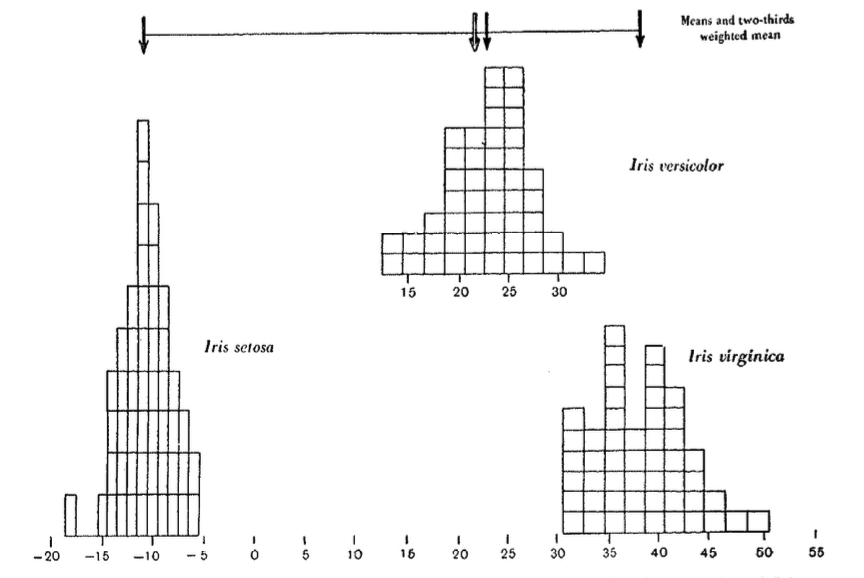
\includegraphics[width=1\linewidth]{img.png}
\caption{Гистограммы частот дискриминирующей линейной функции для трёх видов \textit{Iris}.}
\label{fig:1}
\end{figure}
На диаграмме, рисунок~\ref{fig:1}, показаны фактические распределения составной величины, принятой для отдельных особей трёх измеряемых видов. Как было предсказано выше, заметно, что наблюдается некоторое перекрытие распределений \textit{I. virginica} и \textit{I. versicolor}, так что точная диагностика этих двух видов не может основываться исключительно на этих четырёх измерениях одного цветка, взятого с растения, растущего в природе. Тем не менее, в культуре возможно, что одни лишь измерения обеспечат более полное различение видов.


\section*{Русские названия видов ирисов}
\begin{itemize}
\item \textit{Iris setosa} — Ирис щетинистый
\item \textit{Iris versicolor} — Ирис разноцветный
\item \textit{Iris virginica} — Ирис виргинский
\end{itemize}

\begin{thebibliography}{9}
\bibitem{randolph1934} Randolph, L. F. (1934). ``Chromosome numbers in native American and introduced species and cultivated varieties of Iris.'' \textit{Bull. Amer. Iris Soc.} \textbf{52}, 61--66.
\bibitem{anderson1935} Anderson, Edgar (1935). ``The irises of the Gaspe Peninsula.'' \textit{Bull. Amer. Iris Soc.} \textbf{59}, 2--5.
\bibitem{anderson1936} Anderson, Edgar (1936). ``The species problem in \textit{Iris}.'' \textit{Ann. Mo. Bot. Gdn.} (in press).
\end{thebibliography}


\end{document}